\begin{minipage}[b]{0.6\textwidth}
\begin{Exercise}[label = col1, title = Stoßaufnahme, origin = Aaron Wild, difficulty = 5]
Die nebenstehende Abbildung zeigt die Positionen von zwei Körpern zum Zeitpunkt $t_0$ und $t_1$. Die Körper sind sehr klein, und bewegen sich reibungsfrei auf einem Tisch.\\
Der rote Körper hat eine Masse, die dreimal so groß ist wie die des blauen.\\
Bestimme in der Abbildung (in größerer Form auch auf der nächsten Seite) die Bewegungsrichtungen der beiden Körper, nachdem sie zusammengestoßen sind. Nimm dazu an, dass beide Körpermittelpunkte zum Zeitpunkt des Stoßes auf der Gerade der Bewegungsrichtung des roten Körpers liegen.
\end{Exercise}
\end{minipage}
\begin{minipage}[b]{0.4\textwidth}
	\flushright
	\begin{tikzpicture}
	\filldraw[color =black, fill = blue]  (-2,2.31) circle (2pt);
	\filldraw[color = black, fill = blue] (0,1.155) circle (2pt);
	\filldraw[color = black, fill = red] (0,0) circle (2pt);
	\filldraw[color = black, fill = red] (1,0) circle (2pt);
	\node at (-2,2.7) {$t_0$};
	\node at (0,1.5) {$t_1$};
	\node at (0,-0.5) {$t_0$};
	\node at (1,-0.5){$t_1$};
\end{tikzpicture}
\end{minipage}
\begin{Answer}[ref = col1]
	Die beiden Körper sollen sich geradlinig gleichförmig bewegen. Die Richtung der Geschwindigkeitsvektoren können wir feststellen, indem wir eine Gerade durch die jeweils gegebenen Positionen der beiden Körper legen. \\
	Obwohl wir die Dauer $t_1-t_0$ nicht kennen, reicht es zu wissen, dass sie für die Aufnahmen beider Körper gleich war. Deswegen können wir für diese Aufgabe, in der es uns nur um die Bewegungsrichtungen der beiden Körper nach dem Stoß geht, einfach davon ausgehen, dass die Verbindungen der jeweiligen Körperpositionen unsere Geschwindigkeitsvektoren (\glqq Geschwindigkeitspfeile\grqq) sind, mit denen wir jetzt weiter rechnen können.\\
	Gleichzeitig kennen wir die Massen der beiden Körper nicht, nur deren Verhältnisse. Das ist aber auch nicht weiter schlimm, da während des Stoßes keine Masse verloren geht. Deswegen reicht es, dass gegeben ist, dass der eine Körper dreimal so schwer ist, wie der zweite.\\
	Wenn wir uns jetzt die weitere Bewegung der beiden nach Körper nach $t_1$ anschauen, stellen wir fest, dass die beiden Körper so zusammenstoßen, wie in Abbildung \ref{col1:colfi}
	gezeigt:
	\begin{figure}[h]
		\centering
		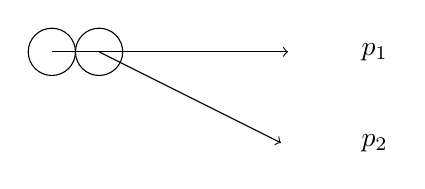
\begin{tikzpicture}
	\draw  (0,0) circle (0.3);
	\draw  (-.6,0) circle (0.3);
	\draw[->] (-0.6,0) -- (2.4,0);
	\draw[->] (0,0) -- (2.31,-1.155);
	\node at (3.5,0) {$p_1$};
	\node at (3.5,-1.155) {$p_2$};
\end{tikzpicture}
		\caption{Geschwindigkeiten und Impulse der beiden Körper direkt vor dem Stoß}
		\label{col1:colfi}
	\end{figure}
	Dabei bezeichnen wir den roten Körper mit einer eins, den blauen mit einer zwei ($m_1 = 3m_2$).\\
	Was wir jetzt machen können, ist zu schauen, entlang welcher Richtung Kräfte bei dem Stoß wirken können, die eine Geschwindigkeitsänderung hervorrufen könnten. Das kann aber nur entlang der Verbindungsline der beiden Körper sein, weil das diejenige ist, an der sich die Berührung der beiden Körper ausrichten muss.\\
	Wenn wir jetzt die Impulse der beiden Körper in eine Komponente entlang dieser $p_\parallel$ Verbindungslinie und senkrecht zu dieser $p_\bot$ aufteilen (siehe Abbildung \ref{col1:colcom}), dann können wir damit sicherlich mehr anfangen:
	\begin{figure}[h]
		\centering
		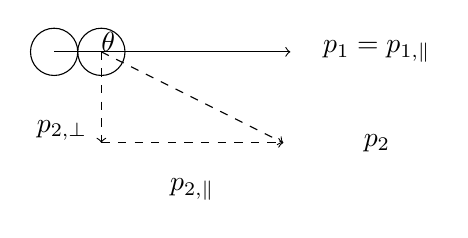
\begin{tikzpicture}
	\draw  (0,0) circle (0.3);
	\draw  (-.6,0) circle (0.3);
	\draw[->] (-0.6,0) -- (2.4,0);
	\draw[->, dashed] (0,0) -- (2.31,-1.155);
	\draw[->, dashed] (0,-1.155) -- (2.31,-1.155);
	\draw[->, dashed] (0,0) -- (0,-1.155);
	\node at (3.5,0) {$p_1 = p_{1,\parallel}$};
	\node at (3.5,-1.155) {$p_2$};
	\node at (-0.5,-1) {$p_{2,\bot}$};
	\node at (1.155,-1.75) {$p_{2,\parallel}$};
	
	\tkzDefPoint(0,0){O}
	\tkzDefPoint(2.4,0){A}
	\tkzDefPoint(2.31,-1.155){B}
	\tkzMarkAngle[scale = 0.85](B,O,A)
	\tkzLabelAngle(B,O,A){$\theta$}
	 
\end{tikzpicture}
		\caption{Impulskomponenten beider Körper direkt vor dem Stoß}
		\label{col1:colcom}
	\end{figure}\\
	Wenn wir den Winkel zwischen den beiden Impulse $\theta$ nennen, dann können wir einfach trigonometrisch schreiben:
	\begin{equation}\label{col1:pcom}
		p_{2,\parallel} = p_2\cos \theta ~\mathrm{und}~p_{2,\bot} = p_2 \sin \theta.
	\end{equation}
	Was bringt uns das jetzt alles? Wir wissen, dass für eine Impulsänderung eine Kraft benötigt wird. Und diese Kraft kann nur entlang der Verbindungsstrecke der beiden Körper wirken. Das heißt aber, dass die Impulskomponenten, die senkrecht auf der Verbindungsstrecke der beiden Körper stehen, durch den Stoß nicht geändert werden könnnen! In diesem Fall ist das zwar \glqq nur \grq{} $p_{2,\bot}$, aber immerhin! Wenn wir die Impulskomponenten nach dem Stoß mit einer Tilde bezeichnen (also die Impulse $\tilde{p}_{1}$ und $\tilde{p}_2$ suchen, die die Komponenten $\tilde{p}_{1,\parallel}$, $\tilde{p}_{1,\bot}$ $,\tilde{p}_{2,\parallel}$ und $\tilde{p}_{2,\bot}$ haben), können wir jetzt zumindest schon schreiben
	\begin{equation}\label{col1:p2on}
		\tilde{p}_{2,\bot} = p_{2,\bot}.
	\end{equation}
	Schön ist jetzt, dass die Impulserhaltung bei einem Stoß sowohl für die senkrecht zur Verbindugsline stehenden Impulskomponenten gilt, als auch (seperat) für die Impulskomponenten entlang der Bewegungsrichtung,
	\begin{equation}\label{col1:pcon}
		p_{1,\parallel} = \tilde{p}_{1,\parallel} + \tilde{p}_{2,\parallel}.
	\end{equation}
	Gleichzeitig können wir die Energieerhaltung schreiben als (mit dem Satz des Pythagoras)\footnote[2]{Wir schreiben die kinetische Energie hier allgemein als $E = \nicefrac{1}{2m}\cdot p^2$. Das erhält man, wenn man $p = m v$ zu $v = \nicefrac{p}{m}$ umstellt, und dann in $E = \nicefrac{1}{2}\cdot mv^2 = \nicefrac{1}{2}\cdot m \left(\nicefrac{p}{m}\right)^2 = \nicefrac{1}{2m}\cdot p^2$ einsetzt.  }
	\begin{equation}\label{col1:encon}
	E = \tilde{E}\Rightarrow	\frac{1}{2m_1} \underbrace{p_{1,\parallel}^2}_{= p_1^2} + \frac{1}{2m_2} \underbrace{\left(p_{2,\bot}^2+p_{2,\parallel}^2\right)}_{=p_2^2} = \frac{1}{2m_1}\tilde{p}_{1,\parallel}^2 + \frac{1}{2m_2}\left(\tilde{p}_{2,\bot}^2+\tilde{p}_{2,\parallel}^2\right) \overset{p_{2,\bot} = \tilde{p}_{2,\bot}}{\Rightarrow} \frac{p_{1,\parallel}^2}{2m_1}   = \frac{\tilde{p}_{1,\parallel}^2}{2m_1}  + \frac{\tilde{p}_{2,\parallel}^2}{2m_2}.
	\end{equation}
	Wenn wir uns jetzt \eqref{col1:pcon} und \eqref{col1:encon} länger anschauen, stellen wir fest, dass alle nur noch Impulskomponenten entlang der Verbindungslinie enthalten (also nur $p_{1,\parallel}$, $\tilde{p}_{1,\parallel}$ und $\tilde{p}_{2,\parallel}$)! \\
	Das heißt, dass wir das komplizierte zweidimensionale Problem (es gab ja sowohl Impulskomponten senkrecht und parallel zur Verbindungslinie) auf ein eindimensionales reduziert haben. Das sollte Sachen viel einfacher machen. \\
	Und am einfachsten wird das Problem, wenn wir es zuerst im sog. Schwerpunktsystem betrachten. Hier ruht der Schwerpunkt der beiden Körper (der sich sonst mit einer konstanten Geschwindigkeit bewegt). \\
	Die Impulskomponenten vor dem Stoß im Schwerpunktsystem sind gegeben durch
	\begin{equation}\label{col1:psps}
		p^{\dagger}_{1,\parallel} = \frac{1}{1+\beta} p_{1,\parallel} - \frac{\beta}{1+\beta} p_{2,\parallel} ~\mathrm{und}~p^{\dagger}_{2,\parallel} = \frac{\beta}{1+\beta}p_{2,\parallel} -  \frac{1}{1+\beta} p_{1,\parallel}.
	\end{equation}
	Wir sehen, dass $p^{\dagger}_{1,\parallel} + p^{\dagger}_{2,\parallel} = 0$ ist, wie erwartet.\\
	Weil der Gesamtimpuls auch im Schwerpunktsystem beim Stoß erhalten bleiben muss, und nach dem Energieerhaltungssatz die absoluten Größen der Impulse auch erhalten bleiben müssen, ist es nach dem Stoß nur möglich, dass sich die Impulse gedreht haben, aber immer noch entgegengesetzt sind. 

	\end{Answer}